\documentclass[11pt,twoside]{report}
\usepackage{preamble}
\graphicspath{{../img/ch2/}}
\setcounter{chapter}{1}


\begin{document}


\chapter{The Collective Behaviour of Animals as Active Matter}
\label{chapter:collective_behaviour}

\epigraph{We declare that the splendour of the world has been enriched by a new beauty: the beauty of speed.}{F. T. Marinetti\\ \emph{Manifesto of Futurism}}

\section{Active Matter}
\label{section:active-matter}

This chapter would discuss the collective behaviour of \emph{active matter}, focusing on the behaviour of \emph{animals}.
The term \emph{active matter} refers to a class of non-equilibrium systems, whose constituting individuals constantly consume energy to generate systematic motion \cite{ramaswamy2017}. These individuals are called \emph{active particles}, and they often propel themselves along the direction of their \emph{orientations} \cite{romanczuk2012}.


\subsection{What is the activity?}


\marginpar{
\centering
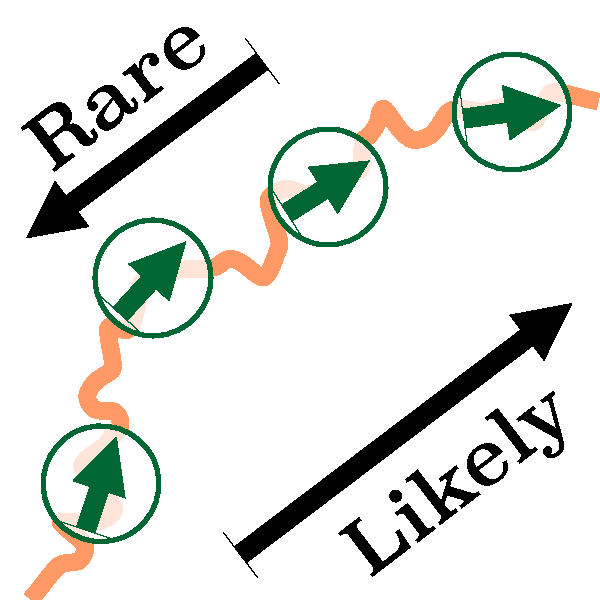
\includegraphics[width=\marginparwidth]{active-trs}
\captionof{figure}[The trajectory of a single active particle]{
	The trajectory of a single active particle, which breaks the time-reversal symmetry. The arrow in the circle represents the orientation of the particle, the direction of the self-propelling force.
}
\label{fig:active-trs}
}


Active particles are different from their passive counterpart in equilibrium systems, because of their ``activity''. The activity could be defined, roughly as the ratio between the deterministic, self-propelling movement, and the stochastic movement from thermal fluctuation.
The self-propelling movement breaks the time-reversal symmetry (\gls{TRS}), making the movement of active particles special \cite{obyrne2022}.
One example of how one active particle breaks the TRS is shown in Fig.~\ref{fig:active-trs}. The self-propelling particle, represented by the circles in Fig.~\ref{fig:active-trs} would have an orientation vector, illustrated by the arrow Fig.~\ref{fig:active-trs}.
This orientational vector is an internal degree of freedom of the particle, like a spin carried by the particle.
The particles would generate motion in the direction of their orientation vector, being self-propelling. An active particle is more likely to form a trajectory, where the particle is always moving along its orientation, rather than moving against its orientation.
For instance, the orange line in Fig.~\ref{fig:active-trs} is more likely to be the trajectory of an active particle that is moving upwards, because the orientations of the particle are pointing at similar directions. It is very unlikely to observe a particle to form such trajectory by traveling from upper right to lower left, if the particle is active\marginfootnote{
It is still possible for the rare situation to happen, but the motion had to be driven by randomness. For instance, an active colloids might move against its propelling force, because of the random kicks from solvent molecules. 
}.
In the absence of activity, where the particle is in equilibrium, the two different options in Fig.~\ref{fig:active-trs} would have the same probability.

The Péclet number (\gls{Pe}) is often used to quantify the activity of the particles \cite{bechinger2016}. It is defined as the ratio between the driven, deterministic motion, and the random, diffusive motion.
It is easy to grasp the effect of activity visually, by inspecting the movement of particles with different Pe values. The trajectories of these particles were plotted in Fig.~\ref{fig:active-trajs}. When $\mathrm{Pe}=0$, the particles perform Brownian motion \cite{rudnick1987}, and they explore a smaller area in the space, having very zigzag and twisted trajectories. As the value of Pe increased, the trajectories appear more straight, and the particles explore more spaces.

\begin{SCfigure}
  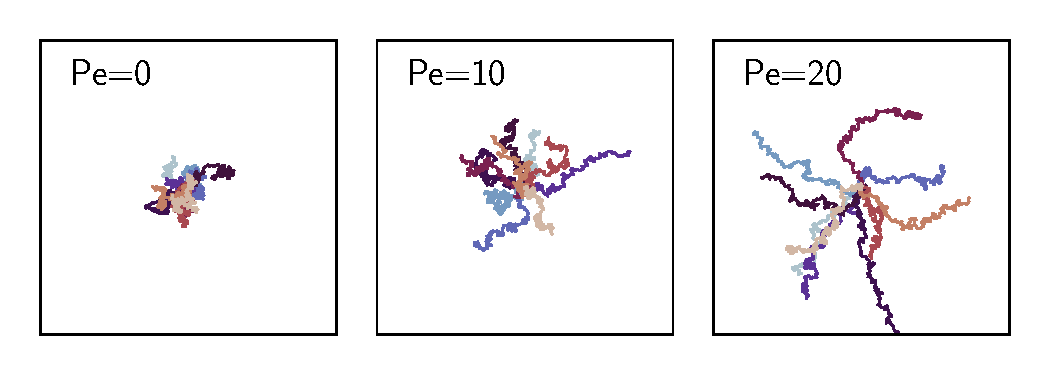
\includegraphics[width=\linewidth]{active-trajs}
  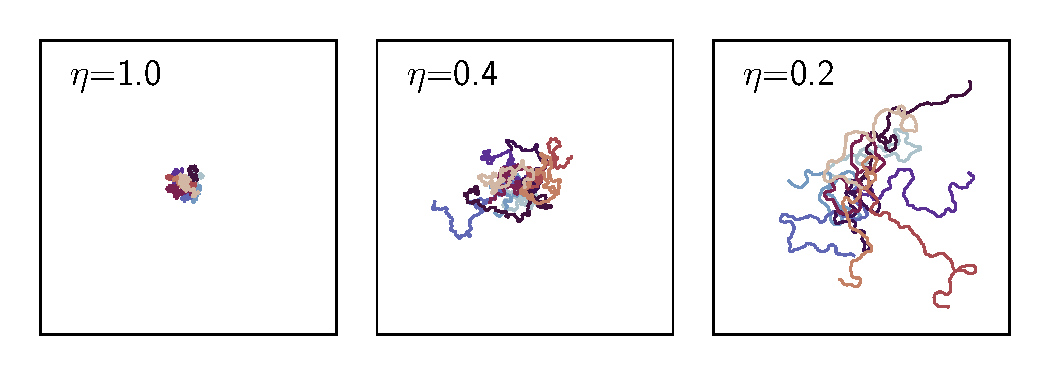
\includegraphics[width=\linewidth]{vicsek-trajs}
  \caption[Trajectories of Active Particles]{
  Trajectories of Active Particles.
  Top: the trajectories of active Brownian particles (ABP) with different Péclet numbers (Pe).
  Bottom: the trajectories of Vicsek agents with different noise ($\eta$) values. 
  Each subplot presents the simulated trajectories of 10 particles.
  }
\label{fig:active-trajs}
\end{SCfigure}


An alternative way to keep track of the activity, is to specify the randomness directly. For instance, we could rotate the moving direction of the active particles randomly, to interrupt their otherwise ballistic self-propelling movement. A system with large noise value therefore would have a low Pe number, hence low activity.
The effect of the noise is shown in Fig.~\ref{fig:active-trajs}. When $\eta = 1$, the rotation is totally random, corresponding to the situation when $\mathrm{Pe}=0$. By reducing the noise, the particles explore more spaces, being more active.\marginfootnote{
It is important to emphasise that the noise term $\eta$ is exclusively used for the Vicsek model, without being referred to as the activity.
}



\subsection{What does active matter do?}
\label{section:active-phase}


The reason we focus on the two aspects of the activity, is related to the two famous models for the active matter. One of the model is the active Brownian particles (\gls{ABP}), where the active particles interact with each other via a short-ranged repulsive interaction. The activity of the active Brownian particles is often represented by the Péclet number \cite{romanczuk2012, mauleon-amieva2020, turci2021}. 
Another widely used model for active matter is the Vicsek model, where the active particles align their orientations with nearby neighbours. The activity of particles in the Vicsek model is often controlled by the noise term \gls{eta} \cite{vicsek1995, gregoire2004, pimentel2008}.

These two models revealed two important phase\marginfootnote{
We committed to follow \citeauthor{toner2005}, calling the \emph{non-equilibrium steady state} with an underlying symmetry a ``phase''.
In the active matter community, this usage of the term ``phase'' is widely accepted.
} behaviours of active matter, which are summarised in Fig.~\ref{fig:active-phase}. 
It is important to stress that the two phase diagrams are sketched in a qualitative way, and some details are ignored. Nevertheless, the phase diagrams are consistent with simulations results, for both 2D and 3D systems \cite{stenhammar2014, turci2021, vicsek1995, solon2015, chate2020}.


\begin{SCfigure}
  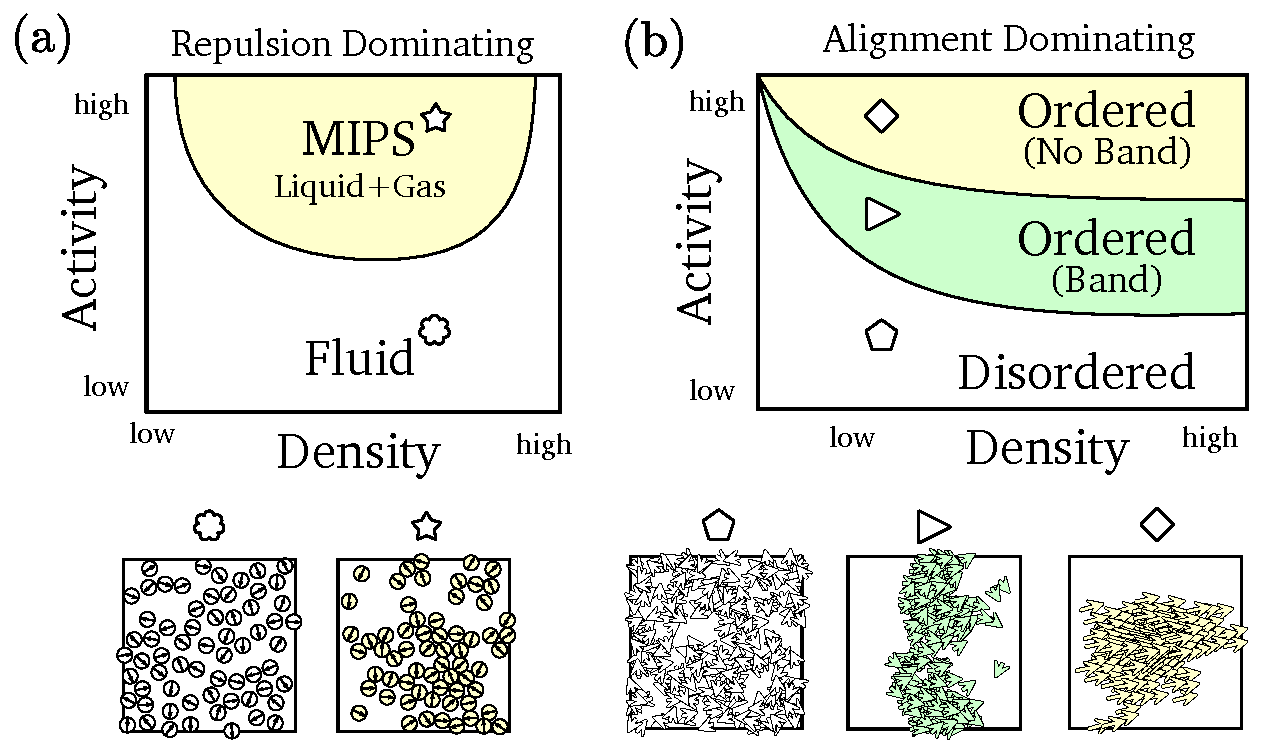
\includegraphics[width=\linewidth]{active-phase}
  \caption[Common phase diagrams of active matter]{
  Two types of common phase diagrams of active matter.
  (a) The phase diagram of active matter systems where the short-range repulsive interaction is dominating. These systems exhibit liquid-gas separation at high level of activity.
  (b) The phase diagram of active matter systems where the velocity-alignment interaction is dominating. These systems exhibit a flocking transition at high activity levels and large density values.
  }
\label{fig:active-phase}
\end{SCfigure}


For the active matter system whose interaction is dominated by short-range repulsion, its behaviour can be summarised in Fig.~\ref{fig:active-phase} (a). While the activity is low, the system forms a fluid with a uniform density distribution, like the behaviour of hard disks (in 2D) \cite{krauth2006, klamser2018, stenhammar2014} or hard spheres (in 3D) \cite{stenhammar2014, robinson2019, turci2021}. 
With high activity values, the active particles begin to phase separate into high density ``liquid'' and low density ``gas'', a phenomena known as the \emph{mobility induced phase separation} (\gls{MIPS}) \cite{fily2012, cates2015, digregorio2018, turci2021}. MIPS is reminiscent of the liquid-gas coexistence in equilibrium systems with attractive interactions \cite{hansen1969, speck2016, anderson2017}. This similarity is indeed surprising: the activity seems to cause an effective attraction between particles \cite{turci2021}. The apparent attractive interaction could be explained by a feedback loop, where the active particles slows down when they accumulate, and the slowing down also induces accumulation of more particles \cite{cates2015}.

On the other hand, for active particles that align their orientation with nearby neighbours, instead of repel each other, their phase behaviour could be summarised in Fig.~\ref{fig:active-phase} (b). In the low activity and low density region, the particles perform disordered movements like the ideal gas. However, with increasing activity and density, the system would undergo an order-disorder transition\marginfootnote{
The transition is also called the \emph{flocking transition} in some literatures \cite{cavagna2020, kürsten2021}. The phenomena where particles perform ordered movement is sometimes called flocking \cite{toner1995, ginelli2010}.
}, where all the particles would share the same moving direction, with slight perturbations from the rotational noise \cite{vicsek1995, solon2015}.
The ordered phase in Fig.~\ref{fig:active-phase} (b) could further be divided into two distinct kinds. When the activity is moderate, the active particles ``travel in bands'' \cite{chate2008}, featuring dense stripes separated by dilute regions, as shown in Fig.~\ref{fig:active-phase} ($\triangleright$). With high activity, the particles do not travel in bands, but rather form a coherent cluster, shown in Fig.~\ref{fig:active-phase} ($\diamond$). The banding phase is an important structural feature of active matter with alignment interactions, which is observed in colloidal experiments \cite{bricard2013, geyer2018, mauleon-amieva2020}.


There are more types of interactions beyond repulsion and alignment. Active matter with more complex interactions exhibits rich behaviours.
For instance, the incorporation of pairwise alignment, short-ranged repulsion, and long-ranged attraction leads to a complex phase behaviour including the fluid, the moving crystal, as well as the polar bands \cite{mauleon-amieva2020}.
The combination of short-ranged repulsion, and dipole-dipole interaction coupled with an alternating current electric field leads to the formation of labyrinth-like patterns \cite{sakai2020}.
In addition, the vision-based acceleration could lead to the formation of a cohesive cluster \cite{lavergne2019}, as a new mechanism beyond of pairwise attraction and MIPS.


It is important to point out that there are topics of active matter that are not covered in this section. For instance, we did not discuss the apolar active matter with nematic alignment interaction \cite{narayan2007, chate2020, bar2020}.
In addition, the effect of activity on the crystallisation \cite{moore2021, omar2021, klamser2018} and glass transition \cite{berthier2017, klongvessa2019} is not discussed.
We also downplayed the importance of dimensionality, which changed the phase diagram of significantly \cite{omar2021, speck2022}.

Finally, we want to specify the meaning following terms, because they were originally developed in equilibrium statistical mechanics. And applying these terms for active matter could cause confusion.

\begin{tcolorbox}[
enlarge bottom by=0.5em,
enlarge top by=0.5em,
]

\begin{description}
	\item [Phase] \hfill \\
	The non-equilibrium steady state with an underlying symmetry, for systems in the thermodynamic limit where the number of particles $\rightarrow \infty$.
	\item [Microscopic State] \hfill \\ Here we refer to the locations, velocities, and orientations of all the active particles. 
	\item [Macroscopic State] \hfill \\ Here we refer to a few global variables, like the density and activity, for an active matter system.
	\item [Collective] \hfill \\ We use the term to specify the property exhibited by a group of animals, in contrast to the property exhibited by individuals.
	\item [Collective Behaviour] \hfill \\ The macroscopic states exhibited by an active matter system.
	\item [Collective Motion] \hfill \\ The microscopic states of an active matter system.\marginfootnote{For a group of fish, we can directly observe their collective motion, and study their collective behaviour by further analysis.}
\end{description}

\end{tcolorbox}

\noindent It is notable that the meaning of these terms is different in different fields. But they will be consistent in this thesis.

\subsection{Animals as Active Matter}

A group of animals is a typical active matter system, as each individual spends their energy to perform movement \cite{ramaswamy2017}.
Consequentially, the two typical phase behaviour of active matter, presented in Fig.~\ref{fig:active-phase}, has been observed in animal groups.
For instance, the MIPS-like behaviour, where a dilute region and a dense region coexist, was observed in a group of beetles \cite{devereux2021}.
In addition, European Starlings exhibit ordered movement \cite{cavagna2010}, while the midges exhibits the disordered movement \cite{attanasi2014pcb}. From a group of zebrafish, we also observed the order-disorder transition \cite{yang2021pcb}, which will be discussed in chapter~\ref{chapter:fish_analysis}.


There is an implicit paradigm to study the active matter system in the scientific community \cite{allen2017}, which includes three steps. Firstly we observe the behaviour of real animals and calculate their behavioural features. Then we simplify the animals with a mathematical model that captured all the essential features \cite{sumpter2012}. Finally we study the model either numerically or analytically, to have a comprehensive understanding. An example of this approach, was recently demonstrated by \citeauthor{bull2021ep3} with a trilogy\marginfootnote{
The authors explained their work in a serious of helpful tweets \cite{prakash2021}. A tweet is a text snippet people posted on a website named ``Twitter''.
}
on the movement of cilia \cite{bull2021ep1, bull2021ep2, bull2021ep3}. It is important to stress that the research on active matter does not always follow the order of ``observation, model, and theory'', even though we will review the literature in such order.


\section{The Observation of Animal Behaviour}
\label{section:intro-observe}

Observing the collective motion of animals is a visually pleasing task, since a group of animals could from striking patterns in nature \cite{vicsek2012}. 
It is expected that animals could do more interesting things, compared with the behaviour of simple active matter systems introduced in section~\ref{section:active-phase}. This is because the interaction between the animal individuals is based on vision \cite{strandburg-peshkin2013}, sound \cite{ota2020}, and smell \cite{miller2022}. All of these biological sensors makes the interaction of animals being more complex than a combination of repulsion and the velocity alignment.

\subsection {Complex Patterns Seen in Nature}

Even the visual footages of the animal behaviour, like the photos and the videos, are useful information.
For instance, the early active matter models were aiming at simulating the movement of animals with visual similarity, rather than quantitative agreement \cite{reynolds1987, vicsek1995, couzin2002}.
Two typical complex patterns commonly seen in the nature were presented in Fig.~\ref{fig:animals}. The first kind is flocking birds, which from a coherent cluster with a smooth but irregular shape (Fig.~\ref{fig:animals}, left subfigure). Another kind of pattern were formed by a school of fish, where the fish rotates around a common axis collectively (Fig.~\ref{fig:animals}, right subfigure), exhibiting a ``milling'' behaviour.

\begin{SCfigure}
  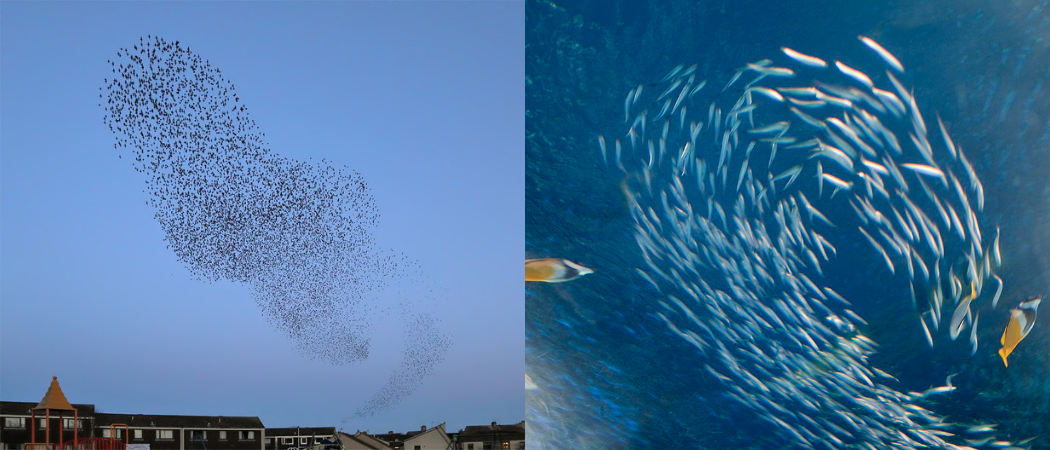
\includegraphics[width=\linewidth]{animals}
  \caption[Complex patterns formed by animals]{
  Photos of complex patterns formed by animals. Both photos were distributed under the Creative Commons Licence.
  Left: the murmuration of flocking European starlings. Each dark dot represents a bird. The photo was taken by \href{https://www.geograph.org.uk/photo/6389346}{Walter Baxter} in Eyemouth, Scotland.
  Right: a school of prey fish forming a circle, as a defensive move against two nearby butterfly fish. The photo was taken by an Internet user named ``\href{http://www.freeimageslive.co.uk/free_stock_image/butterfly-fish-jpg}{lifefish}'', a semi-pro photographer.
  }
  \label{fig:animals}
\end{SCfigure}

\subsection{Observing the Collective Motion in 2D}

To understand the animal behaviour in more detail, it is important to go beyond the visual inspection, and perform quantitative measurement.
One popular option to study animal behaviour is to analyse videos, recorded with conventional cameras, which capture the movement of animals in 2D.
Both the flocking behaviour and the milling behaviour, shown in Fig.~\ref{fig:animals}, were observed from these 2D videos.
For examples, there are analyses on the behaviour of locusts \cite{buhl2006, yates2009}, fish \cite{becco2006, fontaine2008, puckett2018, macgregor2020}, penguins \cite{gerum2013, gerum2018}, and many other animal species \cite{mersch2013, feinerman2018, mendez-valderrama2018, ginelli2015pnas}.


As a well developed experimental technique, the 2D tracking of animals is an easy task. There are multiple free and user-friendly softwares available online, enabling researchers to carry out 2D tracking tasks \cite{perez-escudero2014, rodriguez2017, romero-ferrero2019, walter2021}. The performances of various tracking softwares were quantified in a recent comprehensive review \cite{panadeiro2021}.
In addition to cameras, there are alternative technologies for the study of animal behaviour. For instance, \citeauthor{makris2006} used a waveguide remote-sensing technology to record the density distribution of fish shoals at the scale of kilometers \cite{makris2006, makris2009}.
The GPS is also another option to tag individual animals, and obtain trajectories \cite{papageorgiou2020}.
%For some animals, it is also possible to tag them with informative markers \cite{webster2009, mersch2013, jolles2017}.


\subsection{Observing the Collective Motion in 3D}

The idea of tracking the movement of animals in 3D, with the help of cameras, was proposed early in the 1960s \cite{cullen1965, pitcher1973}.
The fundamental principles to carry 3D tracking were covered by the multiple view geometry in the computer vision community \cite{hartley2003}. Very briefly, the picture in one 2D image offered two constraints on the 3D coordinates of an object. Therefore, 3D coordinates can be determined with images from two or more cameras \cite{cavagna2008ab}. Figure~\ref{fig:locate3d-cartoon} sketched an example for this idea.

\marginpar{
\centering
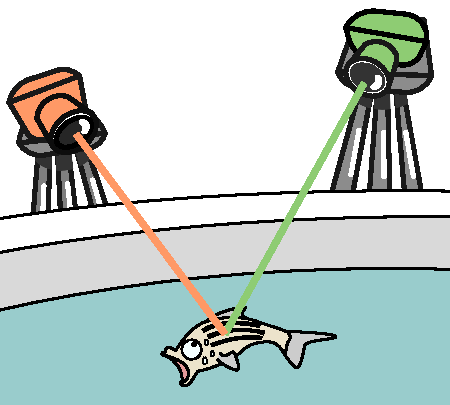
\includegraphics[width=\marginparwidth]{locate3d-cartoon}
\captionof{figure}[Locating a zebrafish in 3D]{
	Schematic illustration for locating a zebrafish in 3D with two cameras. 
}
\label{fig:locate3d-cartoon}
}


Even though the idea is simple, setting up a 3D tracking experiment and obtaining long trajectories of multiple animals are still challenging \cite{pedersen2020}.
Multiple new algorithms have been proposed to tackle the various issues during the tracking process. These issues includes the calibration of camera during field study \cite{cavagna2008ab, ling2018}, the visual occlusions where two animals overlap in the image \cite{cavagna2021ieee}, the ambiguity for the stereo matching of trajectories in multiple views \cite{attanasi2015b}, and the recovery of identity information given the coordinates in different time points \cite{ouellette2005ef, xu2008}.

Despite the technical challenges, the 3D tracking of birds \cite{cavagna2008ab, nagy2010, attanasi2014np, ling2019nee}, insects \cite{butail2011, straw2011, attanasi2014prl, kelley2013, vandervaart2019}, as well as fish \cite{stowers2017, rosa2020, yang2021pcb} were reported.
For the birds, the order ``flocking'' phenomena were observed in \cite{ballerini2008pnas, cavagna2010, nagy2010, ling2018}. For the midges and the fish, the observed movements were disordered \cite{attanasi2014pcb, kelley2013, yang2021pcb}.

There are still two major technical challenges for the 3D animal tracking problem. Firstly, it is very hard to track a large flock of birds for a long time, because the flock would move outside the view of the cameras quickly. This is the reason some of the large scale statistical analysis are only performed on midges \cite{cavagna2017np}, rather than the birds\marginfootnote{
	I was told that the lack of long trajectory is the reason why the author of \cite{cavagna2017np} chose midges over birds.
}.
There is a recent breakthrough to track birds for a long period of time, by moving the cameras in a synchronised fashion \cite{cavagna2021}, but no experimental results were reported from the new system so far.
Another challenge is the 3D tracking of a large school of fish in the sea, which requires underwater equipments. In fact, there is still no quantitative field observation for the a large amount of fish in the milling phase, like those in Fig.~\ref{fig:animals}. Recently, the underwater 3D tracking methods were being developed \cite{francisco2020me, engel2021}, but only for fish groups with small sizes ($N < 10$).


\section{The Analysis of the Collective Motion}
\label{section:intro-analysis}


Analysing the animal movement involves two major steps. 
Firstly, we need to identify the different kinds of behavioural patterns of the animals, and assign the patterns to different phases. For patterns in a particular phase, we can study its feature with different correlation functions.

\subsection{Identifying Behavioural Patterns with \emph{Order Parameters}}
\label{section:intro-order}

This classification of different phases is important, because different phases have different properties.
We can use an \emph{order parameter}, which indicates the breaking of one kind of symmetry \cite{sethna2006}, to identify different phases. For instance, we could define the vector sum of the orientation of each individual as a order parameter ($\mathbf{P}$) \cite{vicsek1995}:

\begin{equation}
	\mathbf{P} = \frac1N \sum_i^N \mathbf{o}_i
\label{eq:pol}
\end{equation}

\noindent where $\mathbf{o}_i$ is the orientation of the $i$th individual in a group with \gls{N} members. We use symbol \gls{pol} to represent the norm of the vector \gls{polvec}. For a very large group, the value of $\Phi$ would approach zero if the orientations of the individuals were completely de-correlated. On the other hand, the value of $\Phi$ would tend to unity if all the individuals have the same orientation. In the latter case, the rotational symmetry is broken because the group has one single moving direction, where the vector $\mathbf{P}$ is pointing at.
The order-disorder transition in Fig.~\ref{fig:active-phase} (b) is characterised by a discontinuous change of $\Phi$. For a flock of birds moving towards the same direction, the value of $\Phi \sim 1$ \cite{attanasi2014np}. For a swarm of randomly moving midges, the value of $\Phi \sim 0$ \cite{attanasi2014pcb}.

\marginpar{
\centering
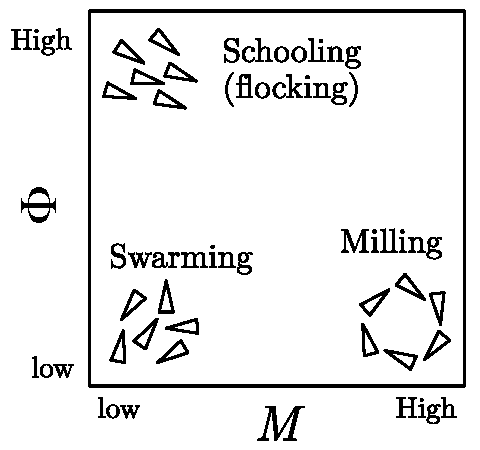
\includegraphics[width=\marginparwidth]{phase-fish}
\captionof{figure}[Different phases revealed by two order parameters.]{
	The schooling, milling, and swarming phases described by  two order parameters. The parameter $\Phi$ indicates the degree of synchronised movement, while the parameter $M$ indicates the existence of collective rotation.
}
\label{fig:phase-fish}
}

The milling behaviour of the fish, shown in Fig.~\ref{fig:animals}, needs a different order parameter that focuses on the angular momentum of each fish. This order parameter is written as,

\begin{equation*}
	\mathbf{M} = \frac1N \sum_i \left(
		\mathbf{o}_i \times \frac{
			\mathbf{r}_i - \mathbf{c}
		}{\vert \mathbf{r}_i - \mathbf{c} \vert}
	\right)
\end{equation*}

\noindent where $\mathbf{r}_i$ represent the location of the $i$th individual, and \gls{center} represents the location of the group centre. Again, we use the symbol \gls{mill} to represent the norm of \gls{millvec}. For a group of fish that are rotating around a common axis, the value of $M$ would be close to one \cite{couzin2002, calovi2014}. For the system that does not perform the collective rotation, the value of $M$ would approach zero.

With the two order parameters, the behavioural pattern of the fish, as well as other species, could be categorised into the swarming, the milling, and the schooling phases, as shown in Fig.~\ref{fig:phase-fish}. The existence of these phases were observed in the a group of golden shiners (\emph{Notemigonus crysoleucas}) \cite{tunstrom2013}.
Operationally, establishing the order parameters helps the identification of the phase that the experimental data (or simulation results) belongs to, without visual inspection.

Inside each phase, we could study its feature by examining the \emph{correlations} in the time and in the space \cite{grigera2020}. The spatial correlations gives us information about the structure of the animal group, while the temporal correlations reveals the dynamics of the system.


\subsection{Probing the Structure: the Radial Distribution Function}
\label{section:intro-corr-rdf}

The radial distribution function (\gls{RDF})\marginfootnote{
The radial distribution function is also named \gls{gr}, which is read as the ``g of r''. We use the term RDF and $g(r)$ interchangeably in this thesis.
} can be used to reveal the structure of the animal group. An example of the RDF, also known as the $g(r)$, is shown in Fig.~\ref{fig:corr-examples} (d). This RDF probes the structural features of a system shown in Fig.~\ref{fig:corr-examples}(a). The value of $g(r)$ at very short range is zero, which represents the short ranged repulsion. The location of the peak of the $g(r)$ is a proxy to the nearest neighbour distance, while the height of the peak indicate the cohesiveness of the group \cite{hansen2013}. The slow decay in Fig.~\ref{fig:corr-examples} shows the presence of large clusters in Fig.~\ref{fig:corr-examples}(a).
The size of these large clusters can be captured by the $r$ value when $g(r)$ decays to zero. This distance value is called \emph{correlation length} of the density \gls{xirho}. 

Notably, the RDF is an important tool for the study of the fluid in equilibrium, because it determines the thermodynamic behaviour of the system \cite{pathria2011, hansen2013}. For instance, the internal energy, the pressure, and the compressibility can be calculated from $g(r)$. However, this validity does not hold for animal groups due to their non-equilibrium nature\marginfootnote{
Recent study suggested that the $g(r)$ can be used to calculate the compressibility for active Brownian particles \cite{dulaney2021}.
}. Nevertheless, the RDF is still a very useful tool to characterise the structure of animal groups, which had been  applied to study the fruit flies \cite{mendez-valderrama2018}, birds \cite{cavagna2008}, the fish \cite{romenskyy2017}, and the penguins \cite{gerum2018}.

Finally it should be mentioned that the $g(r)$ is a two point correlation function, which is not aware of the possible many-body correlations. It was recently revealed by \citeauthor{kursten2020} that higher order correlations are important for the alignment dominating system \cite{kursten2020}, typically the ordered phase in Fig.~\ref{fig:active-phase} (b). The measurements of higher order correlation functions is rare in the study of animal behaviours, but the tools are available in the studies of liquid \cite{zahn2003, williams2007, hallett2020}.
Biologically, the existence of high order structure would be expected. For instance, the formation of the typical V-shape pattern \cite{Hayakawa2013} for a flock of geese could not emerge as a result of simple pairwise interaction.


\begin{SCfigure}
  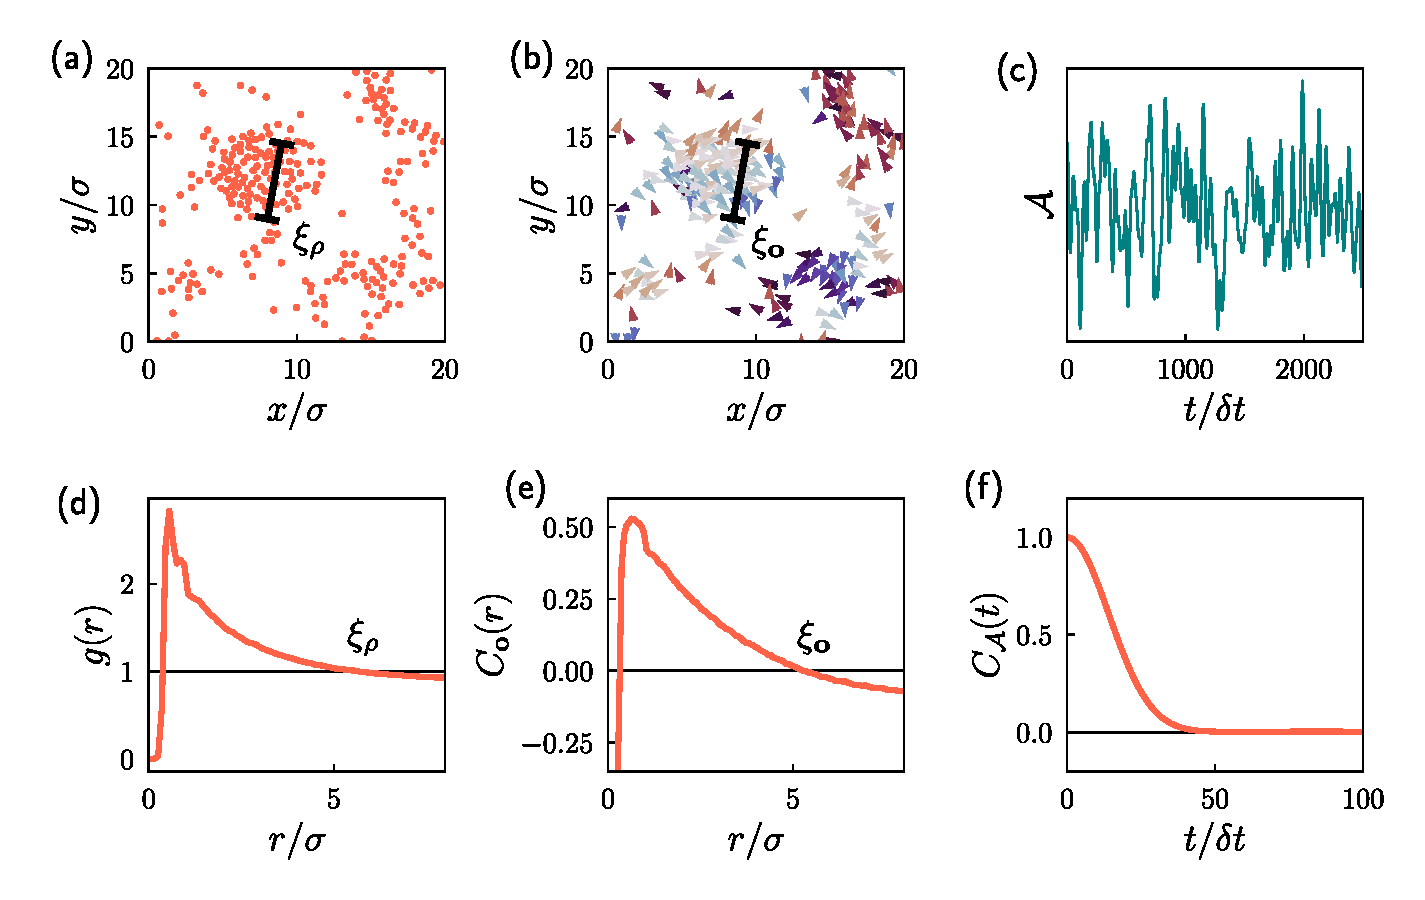
\includegraphics[width=\linewidth]{correlations}
  \caption[Examples of common correlation functions]{
  Examples of common correlation functions and the structure/dynamics that they probe.
  (a) The coordinates of 256 particles with short-ranged repulsion and alignment interaction.
  (b) The orientation of the particles in (a) represented as arrows located at their corresponding coordinates.
  (c) A time series signal of quantity $\mathcal{A}$.
  (d) The radial distribution function ($g(r)$) calculated from the model that generated (a) and (b).
  (e) The connected correlation function of the orientations of particles calculated from the model that generated (a) and (b).
  (f) The auto-correlation function of the signal shown in (c).
  }
  \label{fig:corr-examples}
\end{SCfigure}


\begin{tcolorbox}[
title=Implicit Assumption of the Pairwise Distance $r$,
enlarge bottom by=0.5em,
enlarge top by=0.5em,
]
Using the scalar variable $r$ in a correlation function, we implicitly assumed two conditions. Firstly, the interaction of two particles only depends on their relative distance. In other words, the interaction should be spherically symmetrical. In addition, we assume the system is isotropic with translational symmetry. Therefore, shifting two particles together would not affect their interaction. Without these assumptions, the correlation should be changed from $g(r)$ or \gls{cr} to $g(\mathbf{r}_1, \mathbf{r}_2)$ or $C(\mathbf{r}_1, \mathbf{r}_2)$.
\end{tcolorbox}



\subsection{Probing the Dynamics: the Correlation function of Orientation}
\label{section:intro-corr-cvv}

For a group of animals, as well as other active matter systems, their dynamical features are important. To characterise the dynamics, we can calculate the correlation of the orientations (\gls{o}) of each animal at different distances (\gls{r}). An example of such a correlation function, \gls{cor}, is shown in Fig.~\ref{fig:corr-examples} (e), which characterised the local alignment of particles in Fig.~\ref{fig:corr-examples} (b). These particles are shown to align with nearby neighbours, exhibiting a positive value in the correlation value at short distances. 
%The alignment interaction is short ranged ($= 2\sigma$, where $\sigma$ is the space unit), but it triggered long range correlation, as 
The correlation function reaches 0 at a distance $\approx 5 \sigma$, corresponding to the correlation length of orientation ($\xi_\mathbf{o} = 5\sigma$).
If we compare the correlation functions from both Fig.~\ref{fig:corr-examples} (d) and (e), it is obvious that the two correlation lengths, $\xi_\rho$ and \gls{xio}, are similar. This means the large clusters in Fig.~\ref{fig:corr-examples} (a) and (b) move together, thanks to the local alignment of particles which leads to effective attraction.

Orientational correlation functions are widely applied in the study of animal behaviour, particularly for systems where alignment is the dominating interaction. For instance, the orientational correlation functions of midges \cite{attanasi2014pcb, ni2015epj}, fish \cite{yang2021pcb}, and birds \cite{cavagna2010} have been  reported, presenting short or long ranged orientational correlations.

This function is important also because its integral, $\int C_\mathbf{o}(r) dr$, is related to the \emph{susceptibility} (\gls{chi}) of the animal orientation under an external perturbation, under two assumptions. Firstly, the alignment interaction should dominate the animal behaviour, so that the energy\marginfootnote{
The ``energy'' in Eq.~\ref{eq:spin-energy} ($E: \mathbb{R}^{N \times d} \rightarrow \mathbb{R}$) is effectively a function that maps the \gls{dim} dimensional orientations of $N$ individuals to a probability weight. It is more likely to observe an animal group with a lower energy value.\\
Notice the similarity of Eq.~\ref{eq:spin-energy} to the energy function (the \emph{Hamiltonian}) to those in magnetic systems, for instance the Ising model and the spin glass \cite{castellani2005, herbut2007}.
} of the system \gls{e} follows,

\begin{equation}
	E = -\sum_{i, j}{J_{ij} (\mathbf{o}_i \cdot \mathbf{o}_j})	- 
	h \sum_i{\mathbf{o}_i}
\label{eq:spin-energy}
\end{equation}

\noindent where $\mathbf{o}_i$ is the orientation of the $i$th member in the group, \gls{jij} is a coupling constant for a pair of member $i$ and member $j$, and \gls{h} represents the effect of an external field affecting the individuals' orientations. With the energy term, it is further assumed that the system is in equilibrium, where the entropy is maximised \cite{bialek2011}, so that the probability of the system in a microscopic state with energy $E$ is,

\begin{equation*}
	P(E) = \frac{\exp(-\beta E)}{\int \exp(-\beta E)},
\end{equation*}

\noindent where the integral in the denominator yields the \emph{partition function} of the system. These two assumptions ignored many biological details of the animals, but were confirmed to fit the experimental data \cite{bialek2011}.

Acknowledging the two discussed assumptions, the relationship between $C_\mathbf{o}(r)$ and $\chi = \langle \partial \Phi / \partial h \rangle$ can be derived with the linear response theory\marginfootnote{
	The susceptibility can also be obtained from the fluctuations of the polarisation order parameter ($\vert \mathbf{P} \vert$). Practically, estimating the susceptibility with $\int C_\mathbf{o}(r) dr$ is better for experimental data, because this route suffers less from measurement error and finite trajectory length \cite{attanasi2014prl}.
} \cite{herbut2007, attanasi2014pcb}. The susceptibility is biologically important, because it could be related to the ability of each individuals to change their moving direction, under the influence of a predator (which generates the field $h$ in Eq.~\ref{eq:spin-energy}). And it is been utilised in the study of midges by different research groups \cite{attanasi2014pcb, vandervaart2020}.

\subsection{Probing the Dynamics: the Auto-Correlation Function}
\label{section:intro-corr-acf}

Another way to probe the dynamics of the system is to calculate  the auto-correlation\marginfootnote{
The prefix ``auto'' comes from Greek word autos, which means ``self'' \cite{ben2020}.
} function (\gls{ACF}).
We use the notation \gls{cat} for the ACF for quantity $\mathcal{A}$, whose value typically fluctuates at different time points, like the signal in Fig.~\ref{fig:corr-examples} (c).
The corresponding $C_\mathcal{A}(t)$ is shown in Fig.~\ref{fig:corr-examples} (f), which decays from one to zero. The value of $C_\mathcal{A}(t)$ indicates the average similarity of the signal to itself after some lag time \gls{t}.
The auto-correlation function in Fig.~\ref{fig:corr-examples} (f) indicates that the system forgets its microscopic state, characterised by $\mathcal{A}$, after 50 $\delta t$ (the time unit).
This timescale is called the \emph{relaxation time}, noted by \gls{taua}. Knowing the values of relaxation time for different features let us grasp the dynamics of the system, typically for the identification of fast process and slow process. For instance, the orientational relaxation time of the fruit flies \cite{mendez-valderrama2018} and fish \cite{partridge1981, mwaffo2015, zienkiewicz2015} were estimated from the ACFs.

Beyond the determination of relaxation time, the ACF is important because its integral relates to the transport coefficient, a relation known as the Green-Kubo formula \cite{allen2017, pavliotis2014}. For instance, the integral of the ACF of the velocity (\gls{v}), $\int C_\mathbf{v}(t) dt$ yields the diffusion coefficient. However, this relation requires the collective motion of the animals, treated as a stochastic process, to be second-order stationary, where the ACF does not change with time. In chapter~\ref{chapter:fish_analysis}, we will see that this assumption is not true for the fish, as the \gls{cot} of 50 zebrafish changes with time.


\subsection{Novel Correlation Functions for Animals}
\label{section:intro-corr-special}


It is possible to craft novel correlation functions, like the $g(r)$, to study the structural features of animal groups. For example, \citeauthor{ballerini2008pnas} studied the distribution anisotropy of the neighbours of each bird in a group of European starlings \cite{ballerini2008pnas}. This anisotropy factor, noted as \gls{gamma} in \cite{ballerini2008pnas}, could be used to construct a correlation function $C_\gamma(n)$, with different neighbours rank (\gls{nr}) values\marginfootnote{
For a bird, its nearest neighbour has the rank 1, the next nearest neighbour has the rank 2.

The value of $\gamma$ for the $n$th nearest neighbour is calculated for the entire animal group, in order to quantify the fact, that the neighbours are less likely to be distributed in the moving direction of the group.

Specifically,
$\gamma(n) = \mathbf{w}(n) \cdot \mathbf{P}$.
The vector $\mathbf{w}(n)  \in \mathbb{R}^{m \times 3}$ is the eigenvector of the matrix
$\mathbf{M}(n) = \mathbf{u}(n)^\top \cdot \mathbf{u}(n)$, and $\mathbf{w}(n)$ corresponds to the smallest eigenvalue.
The vector $\mathbf{u}(n) \in \mathbb{R}^{m \times 3}$ stores all the unit vectors pointing from all $m$ birds in the group, to their $n$th closest neighbours.
The vector $\mathbf{P} \in \mathbb{R}^3$ is the polarisation order parameter defined in eq.~\ref{eq:pol}.
}, shown in Fig.~\ref{fig:corr-animal}(a).
This function \gls{cgamman} presents the decay of $\gamma$ with increasing $n$ values, and leads to a remarkable conclusion: a bird in a flocking group interacts with 7 neighbours on average \cite{ballerini2008pnas, cavagna2014}, regardless of its distances to these neighbours.
This behavioural feature is called a \emph{topological} interaction, as opposed to a metric interaction based on physical distances. This special correlation function was also used by \citeauthor{ling2019nc} to study the changing behavioural rules of jackdaw flocks \cite{ling2019nc}.


\begin{SCfigure}
  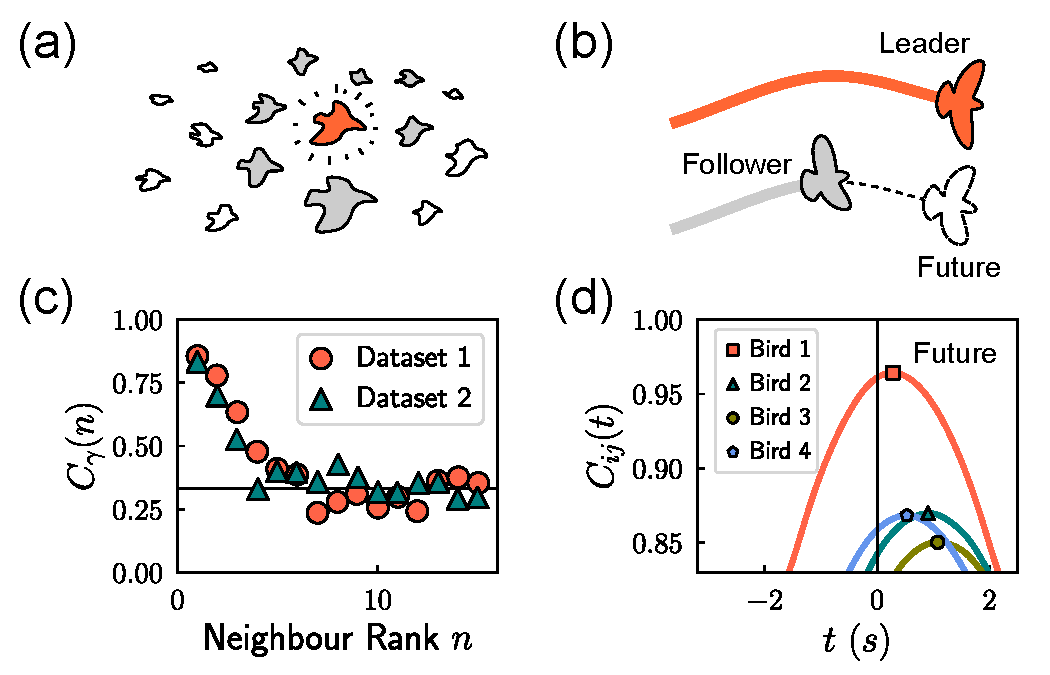
\includegraphics[width=\linewidth]{corr-animal}
  \caption[Examples of special correlation functions to characterise animals]{
Examples of special correlation functions to characterise animals.
  (a) The illustration of a topological interaction, where a highlighted focal bird interact with 7 nearby neighbours, regardless of the distances. This topological interaction is supported by correlation function $C_\gamma(n)$.
  (b) The sketch of a leading bird and a following bird. The following bird will align with the leader, after a short lag time. The leadership is supported by correlation function $C_{ij}(t)$.
  (c) The anisotropy correlation function $C_\gamma(n)$ of the European starlings. The data was obtained from \cite{ballerini2008pnas}.
  (d) The orientational cross-correlation function $C_{ij}(t)$ between a pigeon and its group members. The data was obtained from \cite{nagy2010}.
  }
  \label{fig:corr-animal}
\end{SCfigure}

The correlation function \gls{cijt} is another tool to study animals, proposed by \citeauthor{bumann1993} \cite{bumann1993} in 1990s, and revisited by \citeauthor{nagy2010} in 2010 \cite{nagy2010}. It is essentially the  orientational cross-correlation between two individuals (labelled as $i$ and $j$) in time. Such function revealed the leader-follower relationship among the individuals in the group. An example is plotted in Fig.~\ref{fig:corr-animal} (b), where a following bird would try to align its orientation to a leader. Because of the behavioural inertia of the birds, there will be a slight lag time, for the follower to adjust its orientation. In other words, the follower will try to align with the leader ``now'', but the alignment is not instantaneous, and it could only happen in the ``future''. This lag time could be captured by the orientational cross-correlation function

\begin{equation}
	C_{ij}(t) = \langle
		\mathbf{o}_{i}(\tau) \cdot \mathbf{o}_{j}(\tau + t)
	\rangle,
\end{equation}

\noindent where the angular brackets $\langle \dots \rangle$ represents a time average. Examples of such cross-correlation functions, calculated from pigeons, are shown in Fig.~\ref{fig:corr-animal} (d). For a leading bird, the cross-correlation with its follower would lead to a peak at $t > 0$, because the follower's alignment would happen in the future. This leader-follower relationship of pigeons was also observed by \citeauthor{chen2015epj} \cite{chen2015epj}. And this correlation function as used by \citeauthor{yomosa2013} for the study of gulls \cite{yomosa2013}.

Finally, we want to mention a recent method to quantify the hidden order \cite{martiniani2019prx}, and its correlation length \cite{martiniani2020}. This method used the compression algorithm in computer science to quantify the entropy, as the information with high entropy could not be compressed effectively \cite{mcanlis2016}. This method was demonstrated to be useful for the study of both kind of active matter systems in Fig.~\ref{fig:active-phase} \cite{martiniani2019prx, cavagna2020}.


\section{Understanding the Animal Behaviour}
\label{section:intro-model-theory}

The order parameters, and the correlations calculated from a group of animal can be used to construct mathematical models. These models can be studied numerically or analytically, to make predictive conclusions about the animal behaviour.


\subsection{Microscopic Approach: Agent Based Models}

The most famous model in the active matter community is arguably the Vicsek model proposed by \citeauthor{vicsek1995} in 1995. The model assumed the individual animal in a group align with nearby neighbours. This alignment process is interrupted by the orientational noise ($\eta$ in Fig.~\ref{fig:active-trajs}).
The phase diagram in Fig.~\ref{fig:active-phase} (b) depicted the behaviour of the Vicsek model. The movement of active particles in the ordered phase is visually similar to the collective motion of birds shown in Fig.~\ref{fig:animals} \cite{ballerini2008}.

The Vicsek model is a very simple model, which often lack essential elements to reproduce the behaviour of animals accurately. For instance, the lack of inertia in the Vicsek model makes it incapable of describing the collective turning behaviour of European Starlings \cite{attanasi2014np}. To explain the experimental results, an inertial spin model \cite{attanasi2014np, cavagna2015} was proposed. In addition, the topological interaction rule \cite{ballerini2008pnas}, shown in Fig.~\ref{fig:corr-animal} (a), could also be added into the Vicsek model,  which supressed the travelling bands\marginfootnote{
The existence of the bands for the topological Vicsek model is still under scrutiny. Early results, both simulations and theories, suggested the absence of the band \cite{ginelli2010, chou2012, peshkov2012}. But recent simulations and theories suggested the existence of the band \cite{martin2021, rahmani2021}.
}.


The milling behaviour of the fish \cite{tunstrom2013}, shown in Fig.~\ref{fig:animals} was also modelled by \citeauthor{couzin2002} in early 2000s, known as the Couzin model. This proposed model includes a short ranged repulsion, with an alignment interaction in intermediate range, as well as a long-ranged attraction \cite{couzin2002}. All the phases introduced in Fig.~\ref{fig:phase-fish}, the schooling, milling, and the swarming, can be reproduced in the Couzin model \cite{tunstrom2013}. The same phases could also be reproduced in a model with topological interaction rules \cite{gautrais2012, calovi2014}, as well as a model with only local attraction interactions \cite{strombom2011}.




\subsection{Hydrodynamic Approach: Continuum Models}

One further step to understand the animal behaviour is to convert the microscopic description of the individuals, into large scale, \emph{hydrodynamic} models\marginfootnote{
Also known as the continuum models.
}. By doing so, we ignored the details of the particles, and treat the system as flowing liquid.
This approach is demonstrated by \citeauthor{toner1995}, who derived qualitative predictions for the large scale behaviour of active particles, from hydrodynamic equations.
Typically, these hydrodynamic equations describe the evolution of density field and the polarisation field ($\mathbf{P}$ in Eq.~\ref{eq:pol}), in the form of coupled partial differential equations \cite{toner1995, toner1998, shaebani2019}.
The hydrodynamic description of active matter are expected to recreate the result of the microscopic model at a large-scale \cite{mahault2019}.
The introduction of various continuum models is beyond the scope of this thesis, but we want to discuss some predictive conclusions from theoretical analysis of these models.

The major conclusion from \citeauthor{toner1995} in their early analysis is that the ordered phase discovered by \citeauthor{vicsek1995}, shown in Fig.~\ref{fig:active-phase} (b), exists in 2D. This confirmation is important because the ordered phase could not be proved by numerical simulation in the computer\marginfootnote{
The numerical simulation could generate misleading results, mainly due to the finite system size. For instance, a discontinuous phase transition in the thermodynamic limit ($N \rightarrow \infty$) might appear continuous in a small system ($N \sim 10^4$) \cite{vicsek1995, nagy2006, chate2008EPJ}.
}.
In addition, the analysis carried out by \citeauthor{mermin1966} \cite{mermin1966} explicitly ruled out the possibility for the long ranged order in 2D in equilibrium \cite{sethna2006, ginelli2016}.
In other words, the activity of particles in the Vicsek model is surprisingly crucial for the flocking phenomena.

Beyond the existence of the ordered phase in the 2D Vicsek model (Fig.~\ref{fig:active-phase}), the analysis of the continuum models also yields other useful results such as the scaling of velocity correlation function and the discontinuous nature of the order-disorder transition \cite{solon2015, martin2021}. However, as \citeauthor{ouellette2022} commented recently, it is challenging to link the continuum models to animal groups, especially to compare the theoretical prediction with experimental results, due to the lack of large scale experimental results \cite{ouellette2022}.


\subsection{Thermodynamic Approach: Equation of State}

It is also possible to take a \emph{thermodynamic} approach to study the animal behaviour. Thermodynamics is capable of describing the behaviour of equilibrium systems, whose underlying microscopic dynamics are unknown \cite{ouellette2022}.
For instance, the laws of thermodynamics were established and applied, long before the discovery of atoms and before the development of statistical mechanics \cite{sethna2006, ouellette2022}.
To do something conceptually similar, we will need to define some \emph{state variables}, which are conceptually similar to the pressure (\gls{press}), volume (\gls{vol}), temperature (\gls{temp}), entropy (\gls{entropy}), chemical potential (\gls{mu}) and particle number ($N$), to summarise the behaviour of animals.
If the animals were behaving in an equilibrated way, these state variables would be constrained, yielding an equation of state, that would be useful to develop predictive theories.

For instance, the \emph{virial equation}\marginfootnote{
Notice the law for the ideal gas is $PV = Nk_BT$.
} of an equilibrium system is

\begin{equation}
	 PV = Nk_BT + \langle \mathcal{W} \rangle
\label{eq:virial}
\end{equation}

\noindent where \gls{kb} is the Boltzmann constant, $\langle \dots \rangle$ denotes the time average, and \gls{pressint} is the internal pressure caused by the interaction of particles \cite{hansen2013ch2, allen2017}. Similar relation is observed in \cite{gorbonos2016} for a group of midges, which can be used to calculate the pressure $P$ exerted on the animals by the external field.
In addition, a small perturbation filed acted on the equilibrium system will cause a \emph{linear} response. This linear relationship is observed experimentally in \cite{ni2015prl}.
Further more, \citeauthor{sinhuber2017} were able to observe a constant chemical potential difference between dilute clusters and dense clusters in a swarm of midges, suggesting the existence of phase equilibrium\marginfootnote{
It is important to point out that the chemical potential in \cite{sinhuber2017} took a special definition from \cite{takatori2014}, which depends on the pressure. Again, the pressure in \cite{sinhuber2017} took another special definition, with underlying assumption that the midges were active particles without interaction, and were bounded together by an harmonic potential. Even though the definition of state variables are not very rigorous, their results are still surprising, which should not be discredited.
}.
Remarkably, their experimental results also suggest that detailed balance is maintained, for midges that switch between the two phases \cite{sinhuber2017}.
That is to say, the probability that one midge goes from a dilute region to a dense region, is equal to its counterpart for the reverse process. The detailed balance suggested an equilibrated behaviour of animals at large scale, even though the animal individuals are active and out of equilibrium. This ``regained equilibrium'' at large scales had also been reported from computer simulation \cite{egolf2000}.

Following this path, \citeauthor{sinhuber2021} presented a equation of state for midges, written as

\begin{equation}
	PV^{1.7} = c N T^2
\label{eq:eos-midge}
\end{equation}

\noindent where $c$ is a constant, while $P$ represents an effective pressure, $V$ represents the volume of the convex hull constructed from the animal coordinates, and $T$ represents the effective temperature that links to the second moment of the speed distribution.
Even though this equation contains quantities with heuristic definitions (the $P, V, T$ have special definitions), and fitting parameters obtained from experiments (the value of $c$, and some exponents), it  predicted the changing macroscopic states of midges under different perturbations successfully \cite{sinhuber2021}.

Even though the thermodynamic approach is capable of predicting the macroscopic behaviour the the animals, it is less used compared to other approaches, perhaps for the lack of consensus on the definition of the suitable thermodynamic state variables.
However, it is valuable also from a data science perspective, as a guide for us to project high dimensional data (the phase space) to a low dimensional feature space (the space spanned by few thermodynamic state variables). Such dimensional reduction analysis was also carried out manually \cite{yang2021pcb}, or with machine learning methods\cite{tang2020}, without the thermodynamic inspiration.

\section{Is Active Matter an \emph{Useful} Concept?}
\label{section:intro-benefit}

Physicists mention animals as typical active matter in the literatures \cite{reynolds1987, vicsek1995, chate2008EPJ, chen2015, kürsten2021}, but the biology community rarely acknowledges this perspective \cite{ouellette2022}, except for some ecology literatures \cite{guttal2012, tang2020}. The lack of mutual engagement is understandable, as it is difficult to apply the knowledge of active matter physics to biological topics. For instance, how does the activity affect the fitness of the animal group in a given environment? Would sick animals be less active in the wild? My fish is swimming strangely, does activity help to explain the data? To the best of my knowledge, the answers still remain elusive.

However, there are successful examples that bridge this gap between statistical physics and biology.
For instance, the observation and analysis on the European starlings revealed two unexpected features, the topological interaction \cite{ballerini2008pnas}, and the scale-free correlation \cite{cavagna2010}. These two findings are biological facts, even though their connection to the physiology is still missing \cite{ouellette2022}.

%By monitoring the movement of human bronchial epithelial cells (HBECs), typically their dynamical heterogeneity \cite{berthier2011}, \citeauthor{park2015} linked the (biological) mesenchymal-to-epithelial transition \cite{kalluri2009} to the (physical) unjamming-jamming transition \cite{park2015}. Such linkage is important, because the transition process leads to a collective cellular migration, that is closed related to wound repair, cancer invasion, and common diseases like asthma \cite{park2015}.

In chapter~\ref{chapter:fish_mutation} we will present another attempt, to reduce the gap between the biology and physics. 
Operationally, we studied the behaviour of the mutant fish, whose genetic modification is related to human diseases.
Using the correlation function introduced in section~\ref{section:intro-corr-acf}, we discovered the mutant fish are, surprisingly, more active.
We characterised the collective behaviour of the mutant fish with the order parameter introduced in section~\ref{section:intro-order}.
We then explained the behaviour of mutant fish with a microscopic active matter model, introduced in section~\ref{section:intro-model-theory}.
We hope this is an example that the active matter physics can be \emph{useful}.


\begin{adjustwidth}{0cm}{-5cm}

\begin{tcolorbox}[
fonttitle=\sffamily\Large,
right=0.1\linewidth,
top=5mm,
bottom=5mm,
title=Summary of Chapter 2,
]

\begin{itemize}
	\item We gave a brief introduction on active matter, featuring the following concepts.
	\begin{description}
		\item[Active Matter] \hfill \\ 
		A out-of-equilibrium system, containing active particles which constantly inject energy to the system.
		\item[Activity] \hfill \\ 
		The ratio of deterministic, self-propelling movement and the stochastic movement because of thermal fluctuation. We can increase the activity, by increasing the self-propelling speed, or by reducing the level of randomness.
		\item[Phase Behaviour] \hfill \\
		Active particles could exhibit different phase behaviours under different conditions, for instance the MIPS and the order-disorder transition.
	\end{description}
	\item We reviewed recent progress and challenges in the observation of collective motion of animals. Tracking the 2D movement of animals is an easy task, but the 3D tracking of a large group of animals for a long period of time is still challenging.
	\item We introduced following tools to analyse the collective motion for a group of animals.
	\begin{description}
		\item[Order Parameters]\hfill \\ 
			We can use order parameters to summarise the symmetry of the collective motion of animals.
			Animals could be in different macroscopic states, and these states might belong to different phases, characterised by different order parameters.
		\item[Correlation Functions]\hfill \\
			The different states can be characterised by correlation functions.
	\end{description}
	\item We discussed three ways to model the animal behaviour, in order to get more insights and to create predictive theory.
		\begin{description}
		\item[Microscopic Approach]\hfill \\ 
			Model the behavioural rules for each individual, and predict the animal behaviour with computer simulation.
		\item[Hydrodynamic Approach]\hfill \\
			Model the coupled evolution of the density field, velocity field, and other fields for order parameters. Then predict the animal behaviour by analysing the solutions.
		\item[Thermodynamic Approach]\hfill \\
			Describe the macroscopic state of the animals with thermodynamic state variables, and predict the animal behaviour with the equation of state, which constrains the thermodynamic state variables.
	\end{description}
	\item The linkage between active matter physics and biology is discussed.
\end{itemize}
\end{tcolorbox}

\end{adjustwidth}

\end{document}
